\chapter{Individual Constraints: Fundamentals}
\label{chapter9}
\setcounter{enums}{0}


\noindent The present study suggests the use of ICONS (Individual
CONStraints) as the key means of representing information structure
within the framework of HPSG\is{HPSG} (\citealt{pollard:sag:94}) and
MRS\is{MRS}\is{individual constraints}
(\citealt{copestake:etal:05}).\footnote{The feature \isi{ICONS} was
  originally proposed by Ann Copestake and Dan
  Flickinger,\ia{Copestake, Ann}\ia{Flickinger, Dan} for the purpose
  of capturing semantically relevant connections between individuals
  which are nonetheless not well modeled as elementary predications,
  such as those found in intrasentential anaphora, apposition, and
  nonrestrictive relative clauses.\is{relative clause} Copestake and
  Flickinger suggested that the same mechanism can be used to anchor
  information structure constraints to particular clauses.  In a more
  general system that uses ICONS, the value of \isi{ICONS} would be a
  list of items of type \tdl{icons}, where \tdl{info-str} is a subtype
  of \tdl{icons}.\is{\textit{info-str}} For instance, \citet{song:16}
  represents honorification as a binary relation between referential
  items in dialogue via ICONS.} \myS{2:sec:mrs} goes over the basic
skeletons of Minimal Recursion Semantics.  \myS{9:sec:motivations}
offers the basic necessities for using \isi{ICONS} in processing
information structure. \myS{9:sec:info-str}, \myS{9:ssec:mkg}, and
\myS{9:ssec:sform} propose three type hierarchies that place
constraints on information structure semantically and
morphosyntactically.  \myS{9:sec:graph} presents a simplified version
of representation for ease of exposition.




\section{Minimal Recursion Semantics}
\label{2:sec:mrs}


MRS (Minimal Recursion Semantics\is{MRS}
(\citealt{copestake:etal:05}), or sometimes called Meaning
Representation System) is a framework for computational modeling of
semantic representation.  The current work represents information
structure in MRS via \isi{ICONS} (Individual
CONStraints).\is{individual constraints} That is, representation of
information structure is incorporated into MRS (Meaning Representation
System, in this context).  This is an important departure from
previous work in which MRS was conceived as a (possibly
underspecified) representation of a truth-condition associated with a
sentence.\is{underspecification}



There are two distinct characteristics of MRS representations: First,
MRS introduces a flat representation expressing meanings by feature
structures.  Second, MRS takes advantage of \isi{underspecification}
(for handling quantifier scopes and other phenomena),\is{quantifier}
which allows for flexibility in representation.  In MRS description,
it is important to represent the meanings of a sentence in an
efficient manner for a practical purpose.  The main criteria MRS is
grounded upon are as follows.

\myexe{\eenumsentence{\label{def:mrs}
\item Expressive Adequacy: The framework must allow linguistic
  meanings to be expressed correctly.
\item Grammatical Compatibility: Semantic representations must be
  linked cleanly to other kinds of grammatical information (most
  notably syntax).
\item Computational Tractability: It must be possible to process
  meanings and to check semantic equivalence efficiently and to
  express relationships between semantic representations
  straightforwardly.
\item Underspecifiability: Semantic representations should allow
  \isi{underspecification} (leaving semantic distinctions unresolved), in
  such a way as to allow flexible, monotonic resolution of such
  partial semantic
  representations. \citep[p.\ 281--282]{copestake:etal:05}}}



The minimal components of MRS include HOOK, RELS, and HCONS as shown
in \myref{avm:mrs-min}. 


\myexe{\enumsentence{\label{avm:mrs-min}
\begin{tabular}[t]{llll}
\evnup{a.} & \evnup{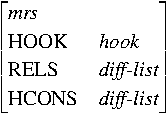
\includegraphics{pdf/mrs-min.pdf}} \\
\evnup{b.} & \evnup{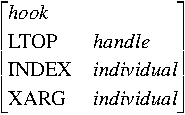
\includegraphics{pdf/hook-min.pdf}} \\ 
\evnup{c.} & \evnup{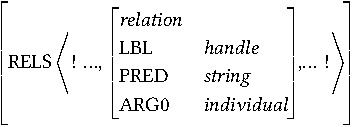
\includegraphics{pdf/rels-min.pdf}} \\
\evnup{d.} & \evnup{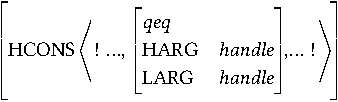
\includegraphics{pdf/hcons-min.pdf}} \\ 
\end{tabular}}}


\noindent First of all, note that AVMs in \myref{avm:mrs-min}, in
which a difference list (i.e.\ \tdl{diff-list}) is used as the value
of RELS and HCONS, are the grammar-internal representations of MRS as
feature structures.\is{MRS}  When MRSs are used as an interface
representation, they use \tdl{list} rather than \tdl{diff-list}, and
do not involve feature structures. Second, HOOK keeps track of the
attributes that need to be externally visible upon semantic
composition, whose minimal components are included in
(\ref{avm:mrs-min}b). The value of LTOP (Local TOP) is the handle of
the relation or relations with the widest fixed scope within the
constituent. The value of INDEX is the index that a word or phrase
combining with this constituent might need access to. The value of ARG
(external ARGument) is identified with the index of a semantic
argument which serves as the subject in raising and control
constructions.\is{raising predicate}\is{control predicate}
Third, REL is a bag of EPs (Elementary Predicates),
whose type is a \tdl{relation}. Each \tdl{relation} has at least three
attributes: LBL (Label), PR ED (Predicate), and ARG0 (ARGument
\#0). The value of LBL is a \tdl{handle}, which represents the current
EP. The value of PRED is normally a string, such as
`\_dog\_n\_1\_rel', `\_bark\_v\_rel', etc.\footnote{The PRED value can
  be a type, particularly for incorporating lexical semantics
  (i.e.\ wordnet) into the meaning representation. Besides, even
  though the PRED value is treated as a string, it is structured.}
The value of ARG0 is either \tdl{ref-ind} for EPs introduced by
nominals or \tdl{event-ind} for EPs introduced by verbals, adjectives,
adverbs, and adpositions.\is{adposition}  Depending on the semantic argument
structure of an EP, more ARGs can be introduced. For example,
intransitive verbs (e.g.\ \textit{bark}) additionally have ARG1,
transitive verbs (e.g.\ \textit{chase}) have ARG1 and ARG2, and
ditransitive verbs (e.g.\ \textit{give}) have ARG1, ARG2, and
ARG3. Finally, HCONS represents partial information about scope.  The
value of HCONS is a bag of \tdl{qeq} (equality modulo quantifier)
constraints.


More recently, alternative representations of MRS have been suggested
for ease of utilizing the MRS formalism for a variety of language
applications, which include RMRS (Robust MRS, \citealt{copestake:07}),
and DMRS (Dependency MRS, \citealt{copestake:09}).  RMRS involves the
functionality of \isi{underspecification} of relational information,
which facilitates shallow techniques in language processing (e.g.\ NP
chunking).  DMRS makes use of a dependency style representation
designed to facilitate machine learning algorithms. It mainly aims to
remove redundancies that (R)MRS may have \citep{eveleigh:10}.  The
current work makes use of the conventional version of MRS, but the
dependency style representation DMRS deploys is introduced for ease of
explication.



\section{Motivations}
\label{9:sec:motivations}

The use of \isi{ICONS} is motivated by three necessities; (i)
resolving discrepancies between forms and meanings in information
structure, (ii) facilitating underspecifiability in order to allow for
flexible and partial constraints, and (iii) capturing the fact that
information structure relations between expressions and particular
clauses.  To these, I add a working hypothesis to facilitate (iv)
informative emptiness in representing information structure.



\subsection{Morphosyntactic Markings \vs Semantic Representation}
\label{9:ssec:ms-vs-sr}

First, the morphosyntactic markings for information structure need to
be kept distinct from semantic markings. This is analogous to the
linguistic fact that morphological tense can sometimes differ from
semantic tense (as exemplified before in counterfactual
constructions \mypage{exe:iatridou}). Some forms of expressing
information structure do indeed directly indicate specific information
structure roles such as \isi{topic}, \isi{focus}, and \isi{contrast}. For instance, the
contrastive topic marker \textit{th{\`i}} in \ili{Vietnamese} directly
assigns \isi{contrastive topic} meaning to the NP that the marker is
attached to, as repeatedly exemplified below.

\myexe{\enumsentence{\label{exe:vie:ch9}
\shortex{4}
  {Nam & th{\`i} & {\textcrd}i & H\`{a} N\textsubdot{\^{o}}i}
  {Nam & \textsc{thi} & go & Ha Noi}
  {`Nam goes to Hanoi(, but nobody else).' [vie] \citep[p.\ 1]{nguyen:06}}}}

\noindent A specific sentence position can also play the same
role. For example, if the word order is not neutral in \ili{Russian},
the clause-final position assigns the non-contrastive \isi{focus}
meaning,\is{clause-final} while \isi{preposing} is responsible for
\isi{contrastive focus} meaning \citep{neeleman:titov:09}. Yet, quite a few
marking systems do not necessarily reveal which information structure
meanings are being conveyed. The typical case of a discrepancy between
morphosyntactic marking and semantic representation is the information
structure marker \wa in \ili{Japanese} and \nun in \ili{Korean} as
discussed before. Even when a language has a relatively deterministic
relation between forms and meanings, the correlation is neither
perfect nor perfectly understood. For example, the A-accent in
\ili{English} has been widely evaluated as containing \isi{focus} meaning,
but there are some counterexamples to this generalization as
exemplified previously in \myS{4:ssec:conditions} (i.e.\ Second
Occurrence Focus \mypage{exe:fery:krifka:08:sof}). Moreover, there has
been a debate concerning the function of the B-accent, which could
mark (i) just topic \citep{jackendoff:72}, (ii) \isi{contrastive topic}
\citep{kadmon:01,buring:03}, (iii) theme \citep{steedman:00}, and (iv)
\isi{contrast} \citep{hedberg:06}.




\subsection{Underspecification}
\label{9:ssec:underspecification}

Unless there exists a decisive clue to identify the intended
information structure meaning, that meaning is most parsimoniously
represented as underspecified.\is{underspecification}
This proposal is especially crucial for
analyzing sentences which appear in an unmarked word order.  Without
clues to indicate a particular meaning (e.g.\ the \isi{contrastive topic}
marker \textit{th{\`i}} in \ili{Vietnamese}), any constituents in the
unmarked order are not specified for meaning with respect to
information structure. For instance, (\ref{exe:sobaka:ch9}a) presented
again below is in the neutral word order in \ili{Russian}, and the
orthography does not represent prosodic patterns related to
information structure.


\myexe{\eenumsentence{\label{exe:sobaka:ch9}
\item\shortex{2} 
{Sobaka & laet.}
{dog & bark}
{`The dog barks.' [rus]}
\item\shortex{2} 
{Laet & sobaka.}
{bark & dog}
{`The \textsc{dog} barks.' [rus]}}}


\noindent When we do not know which element plays which information
structure role in text-based processing (as in
(\ref{exe:sobaka:ch9}a)), it would be better to leave the information
structure values underspecified allowing for all meanings that the
constituents may potentially have. On the other hand, with in a
sentence like (\ref{exe:sobaka:ch9}b) we can say the \textit{sobaka}
has \isi{focus} meaning because the subject is not \textit{in situ}, and the
inversion serves as the clue for determining focus.


As exemplified hitherto, it is not likely that we can precisely
determine an information structure role of each constituent in many
cases, particularly given that sentence-by-sentence processing usually
lacks discourse-related information.  Hence, it is highly necessary to
represent information structure meanings in a flexible way.  For
instance, note the example in \ili{Greek} (\mypage{exe:greek}), which
is provided again below for the sake of convenience.\footnote{The
  subscript in the original example such as []\mysub{C-Foc}, which
  stands for \isi{contrastive focus}, is removed in \myref{exe:greek:2} in
  order to show the difference between the neutral sentence and the
  marked sentence.}


\myexe{\eenumsentence{\label{exe:greek:2}
\item\shortex{2}
{Thelo & kafe.}
{want.1\textsc{sg} & coffee.\textsc{acc}}
{`I would like coffee.'}
\item\shortex{2}
{Kafe & thelo.}
{coffee.\textsc{acc} & want.1\textsc{sg}}
{`Coffee I would like.' [ell] \citep[p.\ 44]{gryllia:09}}}}


\noindent Because the \isi{postverbal} \isi{focus} \textit{kafe} `coffee' in
(\ref{exe:greek:2}a) takes the object position in the \isi{basic word
  order} and there is no other clue to disclose the information
structure role within the single sentence, it does not have to have
any specific meanings \textit{per se}. That means that \textit{kafe}
in (\ref{exe:greek:2}a) can be evaluated as containing (i)
\isi{non-contrastive focus}, (ii) \isi{contrastive focus}, or even as being (iii)
\isi{background} if the preceding verb \textit{thelo} `want' plays a
focus role. Hence, the semantic representation of \textit{kafe} in
(\ref{exe:greek:2}a) has to cover all those potential meanings
simultaneously (i.e.\ \tdl{non-topic} in the present study).  On the
other hand, the \isi{preverbal} focus in (\ref{exe:greek:2}b)
(\textit{ex situ}) presents a clue indentifying its information
structure meaning.  In other words, \textit{kafe} in
(\ref{exe:greek:2}b) is constructionally marked and thereby conveys a
more specific meaning than that in (\ref{exe:greek:2}a) and it can no
longer be interpreted as background. Nonetheless, its meaning is still
vague allowing for readings as either non-contrastive focus or
contrastive focus. Thus, the ideal representation would be able to
allow for both meanings while still excluding background as a possible
reading (i.e.\ \tdl{focus} as the supertype of both
\tdl{semantic-focus} and \tdl{contrast-focus}).\is{semantic focus}\is{contrastive focus}


\subsection{Binary Relations}
\label{9:ssec:binary}


Third, using \isi{ICONS} is motivated by the necessity of finding
binary relations between a clause and an element uses in the
construction of MRSs)\is{MRS} that belongs to the clause. These binary
relations are crucial in representing the information structure of
various types of utterances.  The typed feature structure of ICONS
consists of three components to identify which element has which
information structure value within which clause.\is{binary relation}


Information structure roles can be represented not as a property of
the constituent itself, but as a relationship that holds between the
clause and the constituent it belongs to. For example, in the \ili{English}
sentence \textit{The \textsc{dog} barks.}, the subject \textit{the
  \textsc{dog}} with the A-accent should be viewed as the the \isi{focus} of
the clause headed by the predicate \textit{barks}, rather than as
simply focused.  This approach is in line with \citet{lambrecht:96}
and \citet{engdahl:vallduvi:96} who regard information structure as a
subtype of sentential grammar.\is{A-accent} That is, whether a
constituent is associated with focus or \isi{topic} should be identified
within the sentence that includes the constituent.


Furthermore, a constituent can have multiple relations with different
clauses. One element can have two (or more) information structure
relations, if it belongs to different clauses simultaneously.  This
notion can be clearly understood if we consider multiclausal
utterances such as those which contain relative and embedded clauses.
Most previous studies on information structure treat only fairly
simple and monoclausal constructions. However, expanding a theory to
include embedded clauses introduces the need to allow a single element
to have multiple information structure meanings.  This is because an
embedded clause not only configures its own information structure, but
also plays an information structure role in the domain of the main
clause that takes the embedded clause as one of the
arguments.\is{relative clause} A typical example of this come from
relative clauses where the antecedent of the relative clauses has
relations with both (i) the verb in the relative clause and (ii) the
other verb in main clause, whose values are not necessarily identical
to each other.



Those kinds of relations have been already captured in an
\isi{LFG}-based study on information structure.\is{relative
  clause}\is{relative pronoun} \citet{bresnan:mchombo:87} argues that
relative pronouns function as the \isi{topic} of relative clauses, following
the theorem presented in \citet{kuno:76}.\footnote{The present study
  does not defer to this argument. \myS{10:ssec:relative} presents the
  details.}  In this analysis, then, relative pronouns are assigned an
information structure value within the relative clause, as shown in
\myref{exe:bresnan:mchombo:87:eng}.


\myexe{\eenumsentence{\toplabel{exe:bresnan:mchombo:87:eng}
\item\evnup{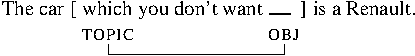
\includegraphics{pdf/bresnan-mchombo-eng-rel.pdf}}
\item\evnup{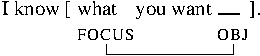
\includegraphics{pdf/bresnan-mchombo-eng-embedded.pdf}}
\item\evnup{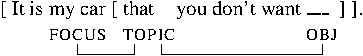
\includegraphics{pdf/bresnan-mchombo-eng-cleft.pdf}} 
\\
\mbox{ } \mbox{ } \mbox{ } \mbox{ } \mbox{ }
\mbox{ } \mbox{ } \mbox{ } \mbox{ } \mbox{ }
\mbox{ } \mbox{ } \mbox{ } \mbox{ } \mbox{ }
\mbox{ } \mbox{ } \mbox{ } \mbox{ } \mbox{ }
\mbox{ } \mbox{ } \mbox{ } \mbox{ } \mbox{ }
  \citep[p.\ 757--758]{bresnan:mchombo:87}}}


\noindent The antecedent corresponding to the relative pronoun
(e.g.\ \textit{the car} in (\ref{exe:bresnan:mchombo:87:eng}a)) has an
additional information structure value within the main
clause.\is{relative pronoun}\is{relative clause} Additionally,
embedded constructions realized as free relative clauses
(e.g.\ \textit{what you want} in (\ref{exe:bresnan:mchombo:87:eng}b))
play yet another information structure role within the main
clause. The clefted NP (e.g.\ \textit{my car} in
(\ref{exe:bresnan:mchombo:87:eng}c)) is assigned a \isi{focus}
meaning,\is{clefting} but its relative pronoun (e.g.\ \textit{that} in
(\ref{exe:bresnan:mchombo:87:eng}c)) plays the \isi{topic} role in the
relative.  While these analyses do not accord perfectly to the
argument presented in the present study, they are still significant
and highlight the necessity of treating information structure as a
relationship between an element and its clause.



\subsection{Informative Emptiness}  
\label{9:sec:hypotheses}


In addition to the motivations presented in the previous subsections,
I provide a working hypothesis about informatively empty categories.
\citet[p.\ 156]{lambrecht:96} argues that expressions which cannot be
stressed, such as expletives (e.g.\ \textit{it} in \textit{It is
  raining.} and \textit{there} in \textit{There is nobody in the
  room.}), unstressed determiners, and so on, cannot be used as \isi{topic}
in principle.  What is to be noted is that they cannot be used for
expressing any other information structure meanings, either.  For this
reason, the present study presents a working hypothesis that
semantically empty categories (e.g.\ complementizers, expletives) and
syncategorematic items\footnote{Syncategorematic items refer to words
  that cannot serve as the main syntactic cateogory of human language
  sentences, such as the subject (in the matrix clause) and the
  predicate.  \citet{lambrecht:96} does not capture any generalization
  about them, but I argue that they cannot be used as topic, either.}
(e.g.\ relative pronouns) are informatively empty as well. This means
no information structure category can be assigned to them, though they
may be required by constructions which serve to mark information
structure, such as the cleft construction in
\ili{English}.\is{clefting}\is{relative pronoun} For example, in
(\ref{exe:void}a), the expletive {\it it} and the \isi{copula} {\it
  is} are semantically empty and the relative pronoun {\it that} is
syncategorematic; thus, they are informatively vacuous. Likewise,
since the copula {\it was} and the preposition {\it by} in
\isi{passive} sentences in English are semantically empty, they cannot
take part in information structure in principle, as shown in
(\ref{exe:void}b).\footnote{In colloquial expressions, copular may
  participate in information structure.  For example, if a question is
  given like \textit{Are you a student?}, then the answer can be
  \textit{I \textsc{was} a student.}  In this case, \isi{focus} is assigned
  to a specific linguistic feature, such as \tdl{tense}, rather than a
  specific constituent.  Admittedly, the current model does not handle
  such a peculiar focus assignment.}  \mysout{Strike} in
\myref{exe:void} indicates that they are informatively meaningless.





\myexe{\eenumsentence{\toplabel{exe:void}
\item{{\Midline{It}} {\Midline{is}} the book {\Midline{that}} was torn
  by Kim.}
\item{The book {\Midline{was}} torn {\Midline{by}} Kim.}}}


\noindent Lexical markers to express information structure, such as
case-marking adpositions (e.g.\ nominative \ga in \ili{Japanese}) are
mostly semantically and informatively empty.\is{adposition} Although
they participate in forming information structure and behave as a clue
for identifying information structure meanings, they do not have their
own predicate names, and do not exist in the semantic representation
(i.e.\ MRS as presented here),\is{MRS} either.  In other words, they
assign no information structure values to themselves, but instead
identify and assign information structure values to the phrase that
they are combined with.  Since the information structure constraints
in the representation of the current work are all relative to elements
in the RELS list, what is not represented in the RELS list cannot bear
any information structure value. In sum, semantically empty lexical
items and syncategorematic items are incapable of bearing their own
information structure value, but they can assign an information
structure value to others.



\subsection{Summary}
\label{9:sec:hierarchies}

The motivations and the working hypothesis presented in this section
are rigorously applied within the remaining parts of this
book. They can be summarized as follows.  

\myexe{\eenumsentence{\toplabel{def:mot:hyp}
\item The formal markings of information structure should be
  modeled separately from the semantic representation of information
  structure.
\item The information structure value should be specified so that it
  can cover all potential information structures that a given sentence
  may have.
\item The semantic representation of information structure involves a
  \isi{binary relation} identifying which element has which
  information structure relation to which clause.
\item Semantically empty and syncategorematic items are informatively
  empty.}}


\noindent These hypotheses are built upon in the following chapters
into three type hierarchies: \tdl{info-str}, \tdl{mkg}, and
\tdl{sform}.\is{\textit{info-str}}\is{\textit{mkg}}\is{\textit{sform}}


\section{Information Structure \textnormal{(}\tdl{info-str}\textnormal{)}}
\label{9:sec:info-str}



\begin{figure}[!t]
\begin{center} 
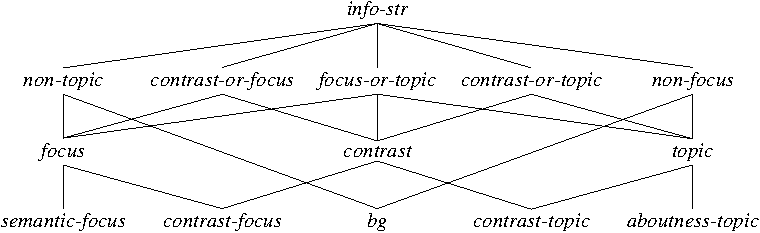
\includegraphics[width=\textwidth]{pdf/info-str.pdf}
\caption{Type hierarchy of \tdl{Info-str}}
\label{fig:info-str}
\end{center}
\end{figure}

\noindent The type hierarchy of \tdl{info-str} is sketched out in
Figure~\ref{fig:info-str}.\is{\textit{info-str}} The values of
information structure are represented as node names (i.e.\ type names)
within the \tdl{info-str} type hierarchy.  For instance, if a
linguistic unit introducing an EP (Elementary Predicate) into RELS is
computed as conveying meaning of \isi{non-contrastive focus}
(i.e.\ \tdl{semantic-focus}), it also introduces one \tdl{info-str}
value whose type name is \tdl{semantic-focus} into ICONS.\is{semantic focus}
The nodes at the bottom represent the most specific meanings, which cannot be
further subdivided with respect to information structure. The nodes in
the third line include the major components of information
structure. \tdl{Focus} and \tdl{topic} are mutually exclusive, and
\tdl{contrast} should be realized with either of them. The nodes in
the second line are abstract. Each of them stands for a linguistic
property that the major components of information structure exhibit:
possibility of topicality or focality (\tdl{non-topic},
\tdl{non-focus}, and \tdl{focus-or-topic}), and possibility of
\isi{contrastiveness} (\tdl{contrast-or-topic} and \tdl{contrast-or-topic}).
These are motivated by the need to capture via
\isi{underspecification} exactly the range of information structure
meanings associated to particular information structure markings in
certain languages, as detailed below.




This \textit{info-str} hierarchy is based on \citet{song:bender:11},
but is extended with several additional nodes. \is{\textit{info-str}}
\tdl{Non-topic} means the target cannot be read as \isi{topic}
(e.g.\ case-marked NPs in \ili{Japanese}).  \tdl{Focus-or-topic} is
assigned to the fronted NPs in focus/topic \isi{fronting} constructions.
\tdl{Contrast-or-topic} is used for \wa in Japanese and \nun in
\ili{Korean}, because \wa or \nun-marked constituents in those
languages can convey a meaning of non-contrastive topic, contrastive
topic, or even contrastive \isi{focus}.  \tdl{Contrast-or-focus} likewise
can be used for forms responsible for a meaning of non-contrastive
focus, contrastive focus, or even contrastive topic.\footnote{Such a
  marking system has not been observed, but it is included into the
  hierarchy as a counterpart of \tdl{contrast-or-topic}.}
\tdl{Non-focus} similarly indicates that the target cannot be the
focus, and would be appropriate for dropped elements in
\textit{pro}-drop languages. As discussed thus far, \tdl{focus} and
\tdl{topic} are mutually exclusive because they designate disjoint
portions of a sentence. \tdl{Focus}, \tdl{contrast}, and \tdl{topic}
multiply inherit from the components in the second row.\is{contrast}\is{focus}
The types in the bottom line represent the fully specified meaning of each
component of information structure.\is{semantic focus} \tdl{Semantic-focus} taken from
\citet{gundel:99} means non-contrastive focus, and
\tdl{aboutness-topic} means non-contrastive \isi{topic}.\is{aboutness topic} Finally, \tdl{bg}
(\isi{background}) means the constituent is neither \tdl{focus} nor
\tdl{topic}, which typically does not involve additional marking but
may be forced by particular positions in a sentence.


Compared to the previous version presented in \citet{song:bender:11}
and other approaches in previous literature, the type hierarchy
illustrated in Figure~\ref{fig:info-str} allows greater
flexibility. First, Figure~\ref{fig:info-str} shows us that
\tdl{contrast}, which is in a sister relation to \tdl{non-topic} and
\tdl{non-focus}, behaves independently of \tdl{topic} and
\tdl{focus}.\is{topic} Second, \tdl{focus-or-topic} and \tdl{contrast-or-topic}
can help in the modeling of the discrepancies between forms and
meanings in information structure (e.g.\ focus/topic \isi{fronting},
\wa or \nun-marked \isi{focus} in \ili{Japanese} and \ili{Korean}, etc.),
and represent ambiguous meanings involving a classification across
\tdl{focus}, \tdl{topic}, and \tdl{contrast}.  Third, \tdl{non-topic}
and \tdl{non-focus} also facilitate more flexible representation for
informatively undetermined items in some languages. For example,
case-marked NPs can convey either focus or \isi{background} meaning of
in Japanese \citep{heycock:94}. That is, since a Japanese case marker
(i.e.\ \textit{ga} for nominatives) can convey two information
structure meanings (\tdl{focus} and \tdl{bg}), the marker itself has
to be less specifically represented as \tdl{non-topic}. Note that
\tdl{non-topic} is the supertype of both \tdl{focus} and
\tdl{bg}. Finally, \tdl{bg} is made use of as an explicit component of
information structure.


Using \isi{ICONS} involves several fundamental points in operation as
follows.  First, \isi{ICONS} represents information structure as a
binary relation between two elements. In other words, the current
model regards \tdl{clause} as the locus where information structure is
determined.\footnote{\mbox{[CLAUSE \tdl{individual}]} and
  \mbox{[CLAUSE-KEY \tdl{event}]} at first blush might look like an
  inconsistency.\is{CLAUSE}\is{CLAUSE-KEY} However, \tdl{event} is a
  subtype of \tdl{individual} in the current type hierarchy of the
  \lingo \isi{Grammar Matrix} system. Roughly speaking,
  \tdl{individual} (an immediate subtype of \tdl{index}) is the lowest
  meaningful supertype of \tdl{ref-ind} for nominals and \tdl{event}
  for verbals.}  Second, \isi{ICONS} behaves analogously to HCONS and
RELS in that values of \tdl{info-str} are gathered up from daughters
to mother up the tree. The value type of ICONS, HCONS, and RELS is
\tdl{diff-list}, which incrementally collects linguistic information
during the formation of parse trees.  Additionally, \isi{ICONS} and
HCONS share almost the same format of feature structure. Both are, so
to speak, accumulator lists. The value type in the \tdl{diff-list} of
\isi{ICONS} is \textit{info-str}, and that of HCONS is \textit{qeq},
both of these include two attributes to represent a \isi{binary
  relation} (i.e.\ TARGET to CLAUSE, and HARG to
LARG).\is{CLAUSE}\is{TARGET} Third, despite the similarity in
structure, RELS and HCONS are different from \isi{ICONS} in terms of
how they function in the semantics.  RELS and HCONS directly engage in
the building up of the logical form, and also interact in an intimate
manner with each other. Although \isi{ICONS} also interact with
truth-conditions \citep{partee:91}, this interaction is not
implemented in the same way.  Fourth, HCONS and ICONS also behave
differently in generation. ICONS-based sentence generation is carried
out via a subsumption check, using the type hierarchy whose value type
is \tdl{icons} or its subtypes
(e.g.\ \tdl{info-str}).\is{\textit{info-str}} That is, the generator
first creates all potential sentences that logically fit in the input
MRS without considering the constraints on ICONS,\is{MRS} and then
postprocesses the intermediate results to filter out sentences
mismatching the values on the \isi{ICONS}
list. Chapter~\ref{chapter12} deals with the details of ICONS-based
generation.



\subsection{ICONS}
\label{9:ssec:icons}


\isi{ICONS} is newly added to structures of type {\it mrs} (i.e.\ under
CONT) as shown in \myref{avm:mrs}.  

\myexe{\enumsentence{\label{avm:mrs}\evnup{
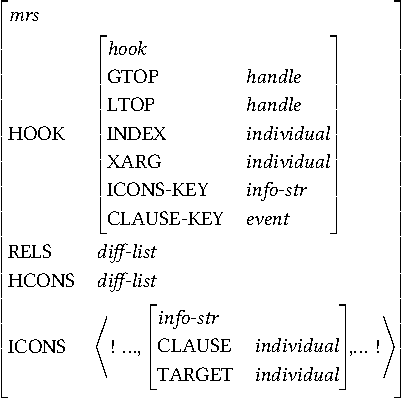
\includegraphics{pdf/icons.pdf}}}}


\noindent An \isi{ICONS} element has two features: namely TARGET and
CLAUSE.\is{CLAUSE}\is{TARGET} When an element is information-structure
marked and also is exhibited as an EP, that element's ARG0 value will
be structure-shared with the value of TARGET.  That is to say, each
type name indicates which information structure meaning is associated
with the EP, and the connection between them is specified by the
co-index between TARGET and ARG0.  On the other hand, the value of
CLAUSE is structure-shared with the INDEX value of the predicate that
functions as the semantic head of the clause.



To take a simple example, (\ref{exe:sample:icons}a) can be represented
as the following AVM (\ref{exe:sample:icons}b).  Note that in
(\ref{exe:sample:icons}a) the subject \textit{\textbf{Kim}} is
B-accented and the object \textit{the \textsc{book}} is
A-accented.\is{A-accent}\is{B-accent}

\myexe{\eenumsentence{\label{exe:sample:icons}
\item{\textbf{Kim} reads the \textsc{book}.}
\item{\evnup{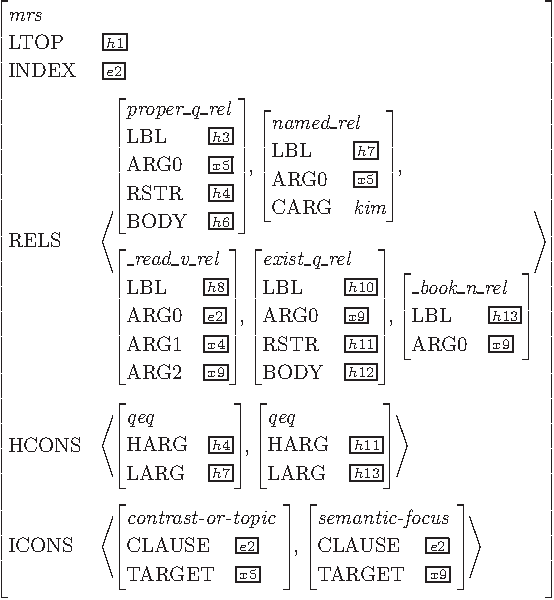
\includegraphics{pdf/sample-mrs.pdf}}}}}


\noindent In (\ref{exe:sample:icons}b), the first element in \isi{ICONS} is
specified as \tdl{contrast-or-topic}, which stands for the information
structure meaning that \textit{\textbf{Kim}} (potentially)
delivers. Likewise, the second element in \isi{ICONS} indicates that
\textit{the \textsc{book}} is evaluated as containing
\tdl{semantic-focus}.\is{semantic focus}  The connection between the elements in ICONS
and the EPs in RELS is determined by the coreference between TARGET of
each \isi{ICONS} element and ARG0 of EP(s). The first element in \isi{ICONS} has
\fbox{\tdl{x5}} for TARGET, and the first and the second EPs in RELS
have the same value. Likewise, the TARGET of the second element in
\isi{ICONS} is co-indexed with the fourth and the fifth EPs' ARG0.\is{CLAUSE} The
values of CLAUSE indicate which EP is the head in the clause. In this
case, the verb \textit{reads} plays the role as indicated by
\fbox{\tdl{e2}}.  The clues to determine information structure
meanings are built up incrementally by lexical and phrasal rules with
an interaction of the type hierarchies. In this case, the rules for
identifying each information structure value are (hypothetical)
lexical rules that constraining the A and B accents.  When a specific
\tdl{info-str} value is created by such a rule, this value is gathered
up to the tree via \tdl{diff-list} \mypage{tdl:diff-list}.


What is key in this method of representation is that the intermediate
types in the hierarchy allow for underspecified representations. As
discussed several times thus far, the grammar of many human languages
does not fully pin down the information structure role an element
plays even when it does provide partial information about it. Because
\tdl{contrast-or-topic} on the first \isi{ICONS} value is not a
terminal node in Figure~\ref{fig:info-str}, \textit{\textbf{Kim}} in
(\ref{exe:sample:icons}a) can be interpreted as any of the categories
subtypes: \tdl{contrast-focus}, \tdl{contrastive-topic},
or \tdl{aboutness-topic}.\is{aboutness topic}\is{contrastive topic}
The specific choice among them can be
determined by the contextual information.  This flexible
representation is crucial in a robust computational model for processing
natural language sentences.








\subsection{ICONS-KEY and CLAUSE-KEY}
\label{9:ssec:icons-key}


In \myref{avm:mrs}, there are two pointers under HOOK; \isi{ICONS-KEY}
and \isi{CLAUSE-KEY}. They are acquired in an incremental way.


ICONS-KEY makes both the phrase/ lexical structure rules and the
lexical entries contribute partial information to the same \isi{ICONS}
element.  When an \tdl{info-str} element can be inserted into the
\isi{ICONS} list, we may not specifically know which information
structure meaning the element carries because information structure
markings often provide only partial information.  The meaning can be
further constrained by multiple sources when the parse tree is further
constructed.  For example, \wa in \ili{Japanese} in itself is assigned
\tdl{contrast-or-topic}, but this meaning can be further constrained
(e.g.\ as \tdl{topic}, \tdl{contrast-topic}, or \tdl{contrast-focus})
by other syntactic operations such as \isi{scrambling}.  Thus, it is
necessary to use a pointer in order to impose a more specific
constraint on an \tdl{info-str} element already augmented in the
\isi{ICONS} list.\is{\textit{info-str}} ICONS-KEY is used for this
purpose.



However, the value of CLAUSE of a constituent cannot be identified
until the clause it belongs to is identified. Thus, when an
\tdl{info-str} element is inserted into the \isi{ICONS} list, the
value of CLAUSE is in most cases not yet specified. This value can be
filled in later by using another pointer called CLAUSE-KEY.  Each
\mbox{ICONS-KEY{$\mid$}CLAUSE} is not lexically bound.\is{CLAUSE} The
value of CLAUSE is naturally identified at the clausal level.  In
other words, the CLAUSE values have to remain unbound until each
clause an individual is overtly expressed in is chosen.\footnote{This
  strategy is different from the approach presented in
  \citet{song:bender:12}, in which \tdl{verbal-lex} and
  \tdl{headed-icons-phrase} take the responsibility of linking
  CLAUSE-KEY to the INDEX of heads. The main reason of the change in
  strategy is that using \tdl{headed-icons-phrase} ends up with
  introducing too many subtypes of
  \tdl{head-comp-phrase}.\is{CLAUSE-KEY} This runs against the spirit
  of the HPSG\is{HPSG} formalism (i.e.\ reducing redundancy and using
  a minimal number of grammatical types).} There are two assumptions
to be noted. The first is that individuals play an information
structure role only with respect to overt clauses.  That is, if an
utterance contains no items that can play a role of the semantic head,
the utterance is assumed to have no CLAUSE binding.\footnote{There are
  some utterances in which no verbal item is used in human language.
  First, if an utterance is vocative (e.g.\ \textit{Madam!}), the
  information structure value of the entire utterance can be evaluated
  as \tdl{focus}.  Second, in languages that do not make use of
  \isi{copula} (e.g.\ \ili{Russian}) copula constructions include
  non-verbal predicates. In this case, since the complement plays the
  semantic head role, the value of CLAUSE is bound to the complement.}
The second is that clauses in this context do not include non-finite
(i.e.\ tenseless) clauses. That is, whether or not a verbal type has a
clausal dependent (subject or complement) is dependent upon whether or
not the dependent involves a verb for which a tense is identified. The
underlined VPs in \myref{exe:PRO} are not clausal arguments. In other
words, the number of clauses in an utterance is the same as the number
of tensed VPs in the utterance.


\myexe{\eenumsentence{\label{exe:PRO}
\item Kim seems \underline{to sleep}.
\item Kim tried \underline{to sleep}.
\item Kim saw Fido \underline{sleeping}.
\item Kim made Fido \underline{sleep}.
\item Kim promised Lee \underline{to leave}. 
\item Kim believed Lee \underline{to have left}.}}


The framework of the \lingo \isi{Grammar Matrix} employs a type hierarchy
representing clausal types, as sketched out in \myref{fig:clause}. The
\tdl{clause} hierarchy is already implemented in the core of the
\lingo Grammar Matrix system (i.e.\ \texttt{matrix.tdl}).


\myexe{\enumsentence{\label{fig:clause}\evnup{
      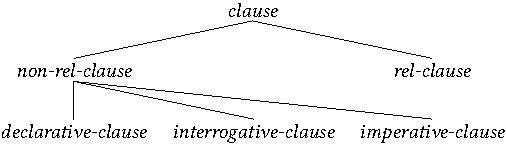
\includegraphics{pdf/clause.pdf}}}}



\noindent Among the nodes in \myref{fig:clause}, \tdl{non-rel-clause}
and \tdl{rel-clause} are responsible for constraining the CLAUSE
values.  The CLAUSE values of the elements on the \isi{ICONS} list
become co-indexed with the INDEX of the semantic head of the CLAUSE
(i.e.\ the value of INDEX being structure-shared with the value of
ARG0 of some EP whose label is the value of LTOP).  This constraint on
\tdl{non-rel-clause} is represented in \myref{avm:non-rel-cl}, in
which CLAUSE-KEY is identified with its INDEX.
 
\myexe{\enumsentence{\label{avm:non-rel-cl}\evnup{
      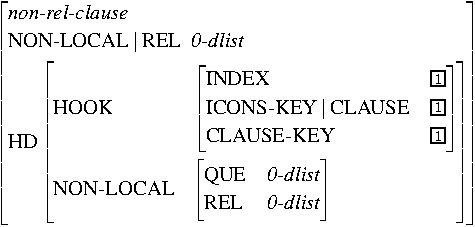
\includegraphics{pdf/non-rel-clause.pdf}}}}

\noindent Because every element in a single clause shares the same
CLAUSE-KEY,\is{CLAUSE-KEY} this coreference is also applied to all
information structure values' \mbox{ICONS{$\mid$}CLAUSE} in
ICONS.\footnote{The constraint on
  \tdl{non-rel-clause} shown in \myref{avm:non-rel-cl} would be incompatible
  with some interrogative sentences in \ili{Bulgarian}:
  \tdl{0-list} in NON-LOCAL{$\mid$}QUE can cause a problem in
  that Bulgarian employs multiple \isi{\textit{wh}-fronting}
  \citep{grewendorf:01}.  Nonetheless, the constraint on
  \tdl{non-rel-clause} is presented as is, because the current
  proposal focuses on information structure in the \lingo \isi{Grammar
    Matrix}. The \isi{\textit{wh}-fronting} is beyond the scope of the
  present work, but should be addressed in future work.} For instance,
lexical types that have an intransitive argument structure (e.g.\ an
intransitive verb \textit{bark} in \ili{English}) inherit from the type
depicted in AVM \myref{avm:intransitive}.  The CLAUSE-KEY of the
subject is identified with the verb's CLAUSE, but the specific value
is not yet given.\is{CLAUSE}\is{CLAUSE-KEY}



\myexe{\enumsentence{\label{avm:intransitive}\evnup{
        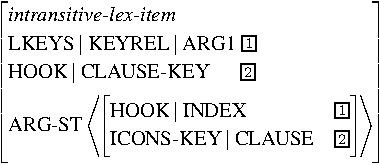
\includegraphics{pdf/intransitive-lex-item.pdf}}}}

\noindent The CLAUSE values (not yet specified) of the elements on the
\isi{ICONS} list are specified when a clause is constructed by
\myref{avm:non-rel-cl}.\is{ICONS-KEY} The same goes for adjuncts in a
single clause.  Adjuncts (e.g.\ attributive adjectives, adverbs, etc.)
and the heads they are modifying share the same value of
CLAUSE.\is{CLAUSE}\is{CLAUSE-KEY} That is, the ICONS-KEY{$\mid$}CLAUSE
and CLAUSE-KEY of NON-HEAD-DTR is identified with the CLAUSE value of
ICONS-KEY of HEAD-DTR. More information about this is given in
\myS{10:sec:monoclausal}
\mypage{avm:head-mod-phrase}.





In \texttt{matrix.tdl} in the \lingo \isi{Grammar Matrix} system, the
subtypes of \tdl{head-subj-phrase} also inherit from the types at the
bottom in \myref{fig:clause} (e.g.\ \tdl{declarative-clause},
etc.). Hence, the instance types (e.g.\ \tdl{decl-head-subj-phrase}
and \tdl{decl-head-opt-subj-phrase}) naturally bear the constraint
\myref{avm:non-rel-cl}.\is{CLAUSE-KEY} In other words, instances of
\tdl{head-subj-phrase} are responsible for the binding of CLAUSE-KEY.




\subsection{Summary}
\label{9:ssec:icons-summary}

As discussed thus far, in order to see the larger picture of how
information is packaged in an utterance, it is necessary to look at
(i) which element has (ii) which information structure relation to
(iii) which clause. In particular, if an utterance is made up of two
or more clauses, single entity can have an information structure
relation (e.g\ \isi{topic}, \isi{focus}, and so on) with each clause, and those
relations are not necessarily the
same.\is{\textit{info-str}}\is{binary relation} Leveraging binary
relations meets this need specifically TARGET for (i), CLAUSE for
(iii),\is{CLAUSE}\is{TARGET} and a value of \tdl{info-str} (i.e.\ a
node in the type hierarchy) for (ii). The items on the ICONS list are
feature structures of type \textit{info-str}, which indicate which
index (the value of TARGET) has a property of information structure
and with respect to which clause (the value of CLAUSE).  Information
structure meanings conveyed by each individual are represented in MRS
as an element of the \isi{ICONS} list,\is{MRS} which our
\isi{infrastructure} of machine translation can refer to for both
transfer and generation.\is{transfer-based}\is{generation}



\section{Markings \textnormal{(}\tdl{mkg}\textnormal{)}}
\label{9:ssec:mkg}

The information structure marking itself is recorded via a
morphosyntactic feature MKG (MarKinG)\is{MKG}\is{\textit{mkg}} inside
of \mbox{SYNSEM{$\mid$}CAT}, which places lexical and syntactic
constraints on forms expressing information structure meanings.  MKG
features are exclusively concerned with markings of information
structure. They are particularly of use for constraining the
\isi{scrambling} constructions in \ili{Korean} and \ili{Japanese},
which will be deeply analyzed in \myS{10:sec:scrambling}
  \mypage{10:sec:scrambling}. Before delving into those details, the
  present subsection presents the basic functionality of the feature
  structure.


MKG plays two roles in handling information structure; one is
theoretically driven, and the other is practical.  First, MKG
contributes to resolving discrepancies between form and meaning in
information structure. As mentioned earlier, the MKG value reflects
the morphosyntactic marking, but does not necessarily coincide with
the semantic value.  For instance, \wa in \ili{Japanese} and \nun in
\ili{Korean} (as discussed in \myS{5:sec:lex}) can sometimes convey a
contrastive \isi{focus} reading as exemplified in \myref{exe:kor:cf:ch9}:
\textit{ecey-nun} `yesterday-\textsc{nun}' in the answer should be
evaluated as conveying a meaning of contrastive focus.  In this case,
the value of MKG that \textit{ecey-nun} has (under CAT) is \tdl{tp},
but the information structure value in semantic representation is
\tdl{contrast-focus}.


\myexe{\eenumsentence{\label{exe:kor:cf:ch9}
\item[Q:]\shortex{3}
{Kim-i& onul & o-ass-ni?}
{Kim-\textsc{nom} &	today & come-\textsc{pst}-\textsc{int}}
{`Did Kim come today?'}
\item[A:]\shortex{4}
{ani. & (Kim-un) & ecey-nun & o-ass-e.}
{No. &	Kim-\textsc{nun} & yesterday-\textsc{nun} & come-\textsc{pst}-\textsc{decl}}
{`No. Kim came yesterday.' [kor]}}}

\noindent Second, MKG also functions as a flag feature for blocking
overgeneration.  The typical instantiation that might be overgenerated
but for MKG is \tdl{topic-comment} constructions, which the next
subsection elaborates on.\is{topic-comment}


The type \tdl{mkg} is used as the value of the feature MKG, and
introduces two further features, FC (FoCus-marked) and TP
(ToPic-marked).\is{\textit{mkg}}


\begin{figure}[!t]
\begin{center} 
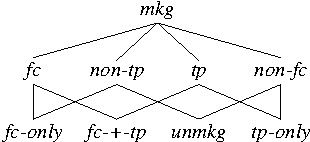
\includegraphics{pdf/hmkg.pdf}
\caption{Type hierarchy of \tdl{Mkg}}
\label{fig:mkg}
\end{center}
\end{figure}


\myexe{\enumsentence{\label{avm:mkg}\evnup{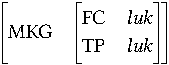
\includegraphics{pdf/mkg.pdf}}}}

\noindent The value type of TP and FC is \tdl{luk}, which is a
supertype of \tdl{bool} (boolean) and \tdl{na} (not-applicable).  As
shown in \myref{avm:mkg}, \tdl{luk} consists of six subtypes including
+, --, and \tdl{na}, and can therefore capture the marking type of
constituents more flexibly than \tdl{bool} which, as shown below, only
has subtypes for + or --.


\myexe{\enumsentence{\label{fig:luk}\evnup{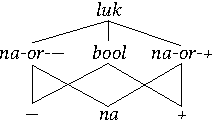
\includegraphics{pdf/luk.pdf}}}}


\noindent The value of MKG\is{MKG} is always a subtype of \tdl{mkg},
as sketched out in Figure~\ref{fig:mkg},\is{\textit{mkg}} in which
\tdl{tp} is constrained as \mbox{[TP +]}, \tdl{non-tp} as
\mbox{[TP \tdl{na-or-${-}$}]}, \tdl{fc} as \mbox{[FC +]}, and
\tdl{non-fc} as \mbox{[FC \tdl{na-or-${-}$}]}. Types at the bottom
multiply inherit from the intermediate supertypes, and thereby both FC
and TP are fully specified.  Instantiations of the \tdl{mkg} values
assigned to particular information structure markings are as follows.


Focus and topic markers in some languages have a fairly
straightforward MKG value. For instance, the contrastive \isi{topic} marker
in \ili{Vietnamese} \textit{th{\`i}} presented in \myref{exe:vie:ch9}
is \mbox{[MKG \tdl{tp-only}]}.  The focus clitics \textit{{\'e}} and
\textit{{\'a}} in \ili{Rendile} exemplified in \mypage{exe:rel} are
\mbox{[MKG \tdl{fc-only}]}. The clitic \textit{=m} in Ingush conveys a
contrastive \isi{focus} meaning \mypage{exe:inh:contrast}, which also
involves \mbox{[MKG \tdl{fc-only}]}. The two types of Cantonese
particles \mypage{exe:man:part}, such as \textit{aa4} for topic and
\textit{aa3} for focus, are \mbox{[MKG \tdl{tp-only}]} and \mbox{[MKG
    \tdl{fc-only}]}, respectively.


The A and B accents in \ili{English}, in line with the analysis in
\citet{hedberg:06}, are also straightforwardly assigned. The A-accent
(H*) is responsible for conveying a non-contrastive \isi{focus} meaning,
whereas the B-accent (L+H*) can be used to express topic (irrespective
of contrastive or non-contrastive) or contrastive focus.\is{B-accent}
\is{A-accent}\is{B-accent} The A-accent exclusively used for marking
focus is \mbox{[MKG \tdl{fc-only}]}, while the B-accent can be left
underspecified with a value like \mbox{[MKG \tdl{tp}]}.




Lexical markers in \ili{Japanese} and \ili{Korean} only partially
constrain meaning. As is well-known, Japanese and Korean employ three
types of NP markings; (i) case-marking (e.g.\ \ga and \ika for
nominatives), (ii) \wa and \nun-marking, and (iii) null-marking
(expressed as {\O}~in the examples presented thus far).\is{lexical
  markers} The distinction among their MKG values is crucially used in
handling the interaction between lexical markings and \isi{scrambling}
in these languages (discussed in detail in
\myS{10:sec:scrambling} \mypage{10:sec:scrambling}).  Initially, the
case markers are \mbox{[MKG \tdl{unmkg}]},\is{MKG} given that they are
not expressly markers of information structure, although they
indirectly influence information structure meanings
(i.e.\ \tdl{non-topic} \citep{heycock:94}). Yet, \tdl{unmkg} does not
necessarily imply a case-marked constituent cannot be used for \isi{focus}
or \isi{topic}. Note that, in the current analysis, information structure
markings are neither a necessary condition nor a sufficient condition
for information structure meanings.  Second, the MKG value of \wa and
\nun may be either \tdl{tp} or a fully specified type such as
\tdl{tp-only}. The present study supports the former, because
contrastively used markers and non-contrastive used ones show
different prosodic behavior from each other in \ili{Korean} and
\ili{Japanese} \citep{chang:02,nakanishi:07}.  For example, as already
provided in Chapter~\ref{chapter8} \mypage{avm:chang:tf},
\citet{chang:02} argues that non-contrastive (`thematic' in his
terminology) \isi{topic} has \mbox{[STR \ensuremath{<1>}]} while contrastive
topic has \mbox{[STR \ensuremath{<3>}]} in Korean.\is{non-contrastive topic}
If we can deploy a
resolution system distinguishing the difference between them in the
future, the value of \mbox{MKG{$\mid$}FC} would not remain
underspecified, and thereby the information structure will be more
concretely constrained.\is{underspecification} In other words, non-contrastively
topic-marked constituents will have \mbox{[MKG \tdl{tp-only}]},
whereas contrastively topic-marked ones will have \mbox{[MKG
    \tdl{fc-+-tp}]}. \tdl{Fc-+-tp} as shown in Figure~\ref{fig:mkg}
means both values of MKG{$\mid$}FC and MKG{$\mid$}TP are +. Note that
these values do not violate the theorem that \isi{focus} and topic are
mutually exclusive.  Since MKG is exclusively concerned with markings,
\tdl{fc-+-tp} does not imply the constituent is regarded as containing
both focus and \isi{topic}.  This value indicates that the constituent is
either focused-marked or topic-marked.  \mbox{[MKG{$\mid$}TP +]} will
come from the lexical information of \nun, and \mbox{[MKG{$\mid$}FC
    +]} will be obtained from the prosodic information of the
constituent (i.e.\ \mbox{[STR \ensuremath{<3>}]}).\is{prosody}
However, a completely reliable system for detecting prosody in
Japanese and Korean, to my knowledge, is non-existent for now.  The
value of MKG{$\mid$}FC of the topic markers, therefore should (and
does) remain underspecified in the current work.  Finally, null-marked
phrases in Japanese and Korean should be evaluated as remaining
underdetermined with respect to information structure markings
(i.e.\ \tdl{unmkg}).\is{underspecification}




The MKG feature also plays a role in calculating the extent of \isi{focus
projection}.\is{prosody} As surveyed in the previous chapter, most
previous HPSG-based analyses of information structure assume that
prosody expressing \isi{focus} is responsible for spreading the meaning of
focus to larger constituents \citep[among many
  others]{bildhauer:07}. However, focus is projected onto larger
phrases not only by means of prosody but also by lexical markers in
some cases \citep{choe:02}.\is{lexical markers} The feature responsibe
for \isi{focus projection} in the current proposal is
\mbox{[MKG{$\mid$}FC +]}.\footnote{The A-accent in \ili{English} and
  the prosodic pattern of marking focus in \ili{Spanish} inherently
  have \mbox{[MKG{$\mid$}FC +]}, which originally comes from
  \mbox{[UT{$\mid$}DTE +]}, if we include \citet{bildhauer:07}'s
  phonological structure and related rules in the
  grammars.\is{A-accent}\is{MKG}}






 




\section{Sentential Forms \textnormal{(}\tdl{sform}\textnormal{)}}
\label{9:ssec:sform}


The value of \isi{ICONS} can be constrained by phrasal types as well
as lexical types.\is{sentential forms}\is{\textit{sform}} In order to
capture a generalization about syntactic combination between two
phrases with respect to information structure, a type hierarchy
representing sentential forms is required. Recall that many previous
studies argue that information structure contributes to a sentential
grammar
\citep{lambrecht:96,engdahl:vallduvi:96,paggio:09,song:bender:11}.
Building on the previous literature, I propose Figure~\ref{fig:sform}
as the classification of phrasal types. The main purpose of
\tdl{sform} is to arrange information structure components in a
sentence.\is{sentential forms} However, this type hierarchy is not
concerned with the linear ordering of components, unlike
Figure~\ref{fig:hier:paggio} given in the previous
chapter \mypage{fig:hier:paggio}.\is{sentential forms}



\begin{figure}[!t]
\begin{center} 
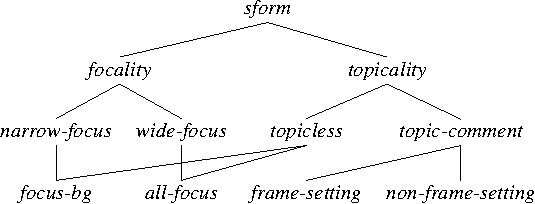
\includegraphics{pdf/sform.pdf}
\caption{Type hierarchy of \tdl{Sform}}
\label{fig:sform}
\end{center}
\end{figure}


\citet{lambrecht:96} posits that information structure is deeply
associated with how a sentence is formed. \citet{engdahl:vallduvi:96},
likewise, regard information structure (information packaging in their
terminology) as a part of sentential grammar. \citet{paggio:09}
provides a hierarchy for representing sentential forms in Danish as
shown in Figure~\ref{fig:hier:paggio},\is{sentential forms} which is
quite similar to Figure~\ref{fig:sform}. \citeauthor{paggio:09}'s type
hierarchy terminates in various phrasal rules that simultaneously
inherit from other fundamental phrasal rules. This method is also
taken up by \citet{song:bender:11}.  In \citeauthor{song:bender:11}'s
analysis of \isi{scrambling} in \ili{Japanese} and \ili{Korean}
(i.e.\ in the OSV order), the combination of scrambled objects and VPs
forms an instance whose type inherits from both \tdl{head-comp-phrase}
and \tdl{topic-comment}.\is{topic-comment} The current model follows the same
combinatoric strategy for placing constraints on phrase structure
types with respect to information structure.


However, there is a methodological difference between what was
proposed in previous literature and that in the present study. In
previous studies the types representing sentential forms also
characterize the linear order of components. For instance, the
instruction-types provided in \citet{engdahl:vallduvi:96}, such as
\tdl{link-focus}, \tdl{link-focus-tail}, \tdl{all-focus}, and
\tdl{focus-tail}, and the node names in the hierarchies of
\citet{paggio:09} and \citet{song:bender:11}, such as
\tdl{topic-focus} and \tdl{topic-bg-focus}, reflect constraints on the
ordering of elements.  In Figure~\ref{fig:sform},\is{sentential forms}
by contrast, only \tdl{topic-comment} is constructed based on linear
order.\is{topic-comment} All the other types merely represent the components that the
construction comprises without respect to the linear
order. \tdl{Focus-bg} in Figure~\ref{fig:sform}, which is normally
used for clefts constructions,\is{clefting} does not mean that
\tdl{focus} is necessarily followed by \tdl{bg}.  For example, focused
constituents are postposed in the cleft constructions in \ili{Korean}
\citep{kim:yang:09}, but these constructions are nonetheless instances
of \tdl{focus-bg}.  In the current work, the linear order of the
components is manipulated by phrase structure rules in each language
grammar.




The types of \tdl{sform} interact with MKG features to stratify
meaning of information structure at the phrase
level.\is{\textit{sform}} The \tdl{sform} types are inherited by
phrase structure rules. Not all phrase structure rules inherit from
\tdl{sform} types, but if a specific syntactic operation is used for
expressing information structure (e.g.\ \isi{scrambling} ins
\ili{Japanese} and \ili{Korean}), the rule for the constructions
inherits from something in Figure~\ref{fig:sform}.



Since sentential forms are basically a matter of how two phrases are
combined with each other,\is{sentential forms} \tdl{sform} inherits
from \tdl{binary-headed-phrase} (made up of HEAD-DTR (head-daughter)
and NON-HEAD-DTR (non-head-daughter)). We may ask why it is necessary
to refer to MKG features of daughters in building up parse trees and
why \tdl{sform} is required to be additionally introduced as a single
phrase structure type.  Several types of constructions use
\tdl{sform}.  Those include (i) the \isi{preverbal}/\isi{postverbal}
position of focused constituents, (ii) cleft
constructions,\is{clefting} (iii) comment markers
(e.g.\ \textit{sh\`{i}} in Mandarin \ili{Chinese} \citep{prince:12}
and \textit{ba} in \ili{Abma} \citep{schneider:09}) that always entail
\isi{focus projection}, and (iv) \isi{scrambling} in \ili{Japanese}
and \ili{Korean} \citep{choi:99,ishihara:01,song:bender:11}. These are
respectively relevant to (i) \tdl{narrow-focus}, (ii) \tdl{focus-bg},
(iii) \tdl{wide-focus}, and (iv) \tdl{topicless} \vs
\tdl{topic-comment}.\is{narrow focus}\is{wide focus}\is{topic-comment}\is{topicless}




\tdl{Sform} is bipartitely divided into \tdl{focality} and
\tdl{topicality}, which indicates marking (i.e.\ values of MKG) and/or
meaning (i.e.\ values of ICONS) of components of information structure
in the arguments.\is{\textit{mkg}}\is{\textit{sform}} \tdl{Sform} and
its subtypes, as presented below, place constraints on MKG,\is{MKG}
which implies sentences are realized depending on information
structure markings of elements.  Since \tdl{sform} also places
constraints on ICONS, it serves to relate the marking to the meaning.


\tdl{Focality} takes \tdl{fc-only} as the value of MKG, which
indicates the phrase includes a \isi{focus}-marked constituent.
\tdl{Focality} is divided into \tdl{narrow-focus} and
\tdl{wide-focus}.\is{narrow focus}\is{wide focus} The distinction between them, however, is not
necessarily equivalent to argument focus \vs predicate focus
\citep{lambrecht:96,erteschik:07}, because verbs can bear
\tdl{narrow-focus}.  As shown in \myref{avm:focality}, only the MKG
value on the mother is restricted in \tdl{focality}. The value is used
for further composition: Some phrase structure rules prevent
focus-marked constituents (i.e.\ specified as \mbox{[MKG{$\mid$}FC
    +]}) from being used as the daughter. Some phrase structure rules,
on the contrary, require an explicitly focus-marked constituent as the
daughter.


\myexe{\enumsentence{\label{avm:focality}\evnup{
      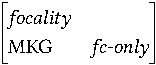
\includegraphics{pdf/focality.pdf}}}}


\tdl{Topicality} is mainly concerned with how the \isi{topic} is realized in
a sentence. \tdl{Topicality} does not have any specific constraint for
now, because \tdl{topicless} and \tdl{topic-comment} are unlikely to
share a feature cross-linguistically.\is{topic-comment}\is{topicless}
Nonetheless, it is introduced
into the hierarchy out of consideration for symmetry with
\tdl{focality}.  Subtypes of \tdl{topicality} are constrained in the
following way.


\myexe{\enumsentence{\toplabel{avm:topicless:topic-comment}
\begin{tabular}[t]{lllll}
a. & \evnup{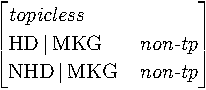
\includegraphics{pdf/topicless.pdf}} & &
b. & \evnup{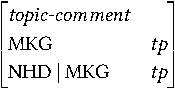
\includegraphics{pdf/topic-comment.pdf}} \\
\end{tabular}}}


\noindent Note that \tdl{topic-comment} has a constraint on the MKG
value of the mother, just as \tdl{focality} above has the constraint
\mbox{[MKG \tdl{fc-only}]}.  In \tdl{topic-comment} constructions
(e.g.\ \textit{as for ...}  constructions),\is{topic-comment} topics are followed by
other constituents. Once a construction is identified as
\tdl{topic-comment}, there are two options in further composition. If
there exists another \isi{topic} in the left side, and the topic is a
\isi{frame-setter}, then further composition is allowed. Otherwise,
the \tdl{topic-comment} instance itself cannot be used as a head
(i.e.\ a secondary \tdl{comment}) in further composition.\is{topic-comment}  The
subtypes of \tdl{topic-comment} (i.e.\ \tdl{frame-setting} and
\tdl{non-frame-setting}) details this
distinction.\is{topic-comment}\is{frame-setting}


As noted, not all sentences have topics.\is{clefting}\is{topicless}
Cleft constructions are presumably \tdl{topicless} in many
languages.\footnote{There exists some exception to this
  generalization. It is reported that some languages
  (e.g. \ili{Spanish}) allow for left-dislocated topics in cleft
  constructions.} Accordingly, a constituent with \mbox{[MKG{$\mid$}TP
    +]} cannot be the non-head-daughter in cleft constructions. For
example, cleft clauses in \ili{Korean} show a strong tendency to be
exclusive to \nun-marked constituents, as exemplified below.


\myexe{\eenumsentence{\label{exe:clefts:kor:ch9}
\item\shortex{5}
  {ku & chayk-ul/*un & ilk-nun & salam-i/un & Kim-i-ta.}
  {the & book-\textsc{acc}/\textsc{nun} & read-\textsc{rel} & person-\textsc{nom}/\textsc{nun}  & Kim-\textsc{cop}-\textsc{decl}}
  {`It is Kim that reads the book.'}
\item\shortex{5}
  {Kim-i/*un & ilk-nun & kes-i/un & ku & chayk-i-ta.}
  {Kim-\textsc{nom}/\textsc{nun} & read-\textsc{rel} & thing-\textsc{nom}/\textsc{nun} & the & book-\textsc{cop}-\textsc{decl}}
  {`It is the book that Kim reads.' [kor]}}}


The distinction between \tdl{topicless} and \tdl{topic-comment} is
especially significant in topic-prominent languages, such as
\ili{Chinese}, \ili{Japanese}, and \ili{Korean}, in which forms of
marking topics play an important role in syntactic configuration
\citep{li:thompson:76,huang:84}.\is{syntactic positioning}
\citet{lambrecht:96} regards \myref{exe:kuroda}, in which \textit{inu}
`dog' is combined with the nominative marker \ga instead of the
so-called \isi{topic} marker \wa, as a topicless
sentence.\footnote{\citet{kuroda:72} regards \myref{exe:kuroda} as a
  subjectless sentence.}  This is further evidence that not all
subjects are topics.\is{topicless}


\myexe{\enumsentence{\label{exe:kuroda}
\shortex{3}
{inu ga & hasitte iru.}
{dog \textsc{nom} & running}
{`The dog is running.' [jpn]  \citep[p.\ 161]{kuroda:72}}}}


\noindent In line with \citeauthor{lambrecht:96}'s claim, the present
analysis provides for this with the type \tdl{topicless}.  The
difference between \tdl{topicless} and \tdl{topic-comment} performs a
role in constructing \ili{Japanese} and \ili{Korean} grammars, which
is partially proposed in \citet{song:bender:11}.\is{topic-comment} For instance,
\tdl{head-subj-rule} and \tdl{head-comp-rule} in these languages need
to be divided into several subrules, depending on whether the
non-head-daughter of the rules are \wa or \nun-marked or not.  The
rules dependent upon the value of MKG in Japanese and Korean are
provided in \myS{10:sec:scrambling}.




There is a need to refine the meaning of \tdl{topicless}.\is{topicless}
On one hand, it indicates that \isi{topic} is not realized in surface form, not that
there is no topic at all in the utterance.  For example,
\tdl{topicless} in \ili{Japanese} means that the non-head-daughter of
the phrase is not \wa-marked.  For example, since \textit{inu ga} `dog
\textsc{nom}' in \myref{exe:kuroda} is not a \wa-marked constituent,
and it constitutes the sentence with the predicate \textit{hasitte
  iru} `running' as a non-head-daughter, the sentence ends up being
\tdl{topicless}.\is{MKG} On the other hand, MKG only reflects overtly
expressed items and an utterance might have an implicit topic which is
not overtly expressed as is the case in \isi{topic-drop}, which often occurs
in topic-prominent languages (e.g., \ili{Chinese}, \ili{Japanese}, \ili{Korean}).
It is true that dropped topics in the current work surely
have a representation in the ICONS, but they are irrelevant to MKG.



\tdl{Narrow-focus} and \tdl{focus-bg} come under \tdl{focality}, but
constraints on them are language-specific.\is{narrow focus} This is because they are
not reflected in the linearization of components. For example, assume
two hypothetical languages Language \textit{A} and \textit{B}, which
have a symmetrical property as follows.\footnote{Language \textit{A}
  is hypothetically modeled quite analogously to Hungarian
  \citep{kiss:98,szendroi:99}. Hungarian is known as adopting SVO word
  order preferentially \citep{gell:ruhlen:11}, though it is sometimes
  reported that the word order in Hungarian is pragmatically
  conditioned (i.e.\ no dominant order \citep{kiefer:67}).}
 

\myexe{\eenumsentence{\label{def:lang-a}
\item Language \textit{A} employs SVO as its \isi{basic word order}.
\item Focused constituents in Language \textit{A} are realized in the immediate
  preverbal position.
\item Additionally, there is an optionally used accent, which
  expresses focus.}}


\myexe{\eenumsentence{\label{def:lang-b}
\item Language \textit{B} employs SOV as its \isi{basic word order}.
\item Focused constituents in Language \textit{B}~ are realized in the
  immediate \isi{postverbal} position.
\item The same as (\ref{def:lang-a}c)}}


\noindent Based on (\ref{def:lang-a}-\ref{def:lang-b}), the object in
SOV word order in Language \textit{A} and the objects in SVO word
order in Language \textit{B} are narrowly focused.\is{narrow focus}
They participate in \tdl{narrow-focus} as a non-head-daughter. Both
[OV] in Language \textit{A} and [VO] in Language \textit{B} are
instantiated as \tdl{head-comp-phrase}, but the former is constrained
by \tdl{head-final} in which the head (i.e.\ the verb) follows its
complement, while the latter is constrained by \tdl{head-initial} in
which the head precedes. Thus, from a cross-linguistic perspective,
linear order does not have to be used as a key to constrain
\tdl{narrow-focus}.\is{narrow focus} On the other hand, a distinction
between HEAD-DTR and NON-HEAD-DTR cannot be used for constraining
\tdl{narrow-focus}, either.  For instance, focused constituents in
clefts behave as the head of cleft clauses realized as
relatives.\is{clefting} In other words, while the focused items in
[OV/VO] in Language \textit{A} and \textit{B} respectively are
non-head-daughters, the focused items in cleft are head-daughters. In
a nutshell, it is true that \tdl{narrow-focus} and \tdl{focus-bg}
require some constraints on information structure marking and meaning,
but the constraints must be applied on a language by language or
construction by construction basis.


There are at least two subtypes of \tdl{focus-bg} across languages:
One where the HD involves [MKG \tdl{fc}] and one where the NHD does.
For example, the cleft constructions (as an instance of
\tdl{focus-bg}) in \ili{English} basically inherit the following
AVM. More specific constraints can be imposed
language-specifically.\is{clefting}

\myexe{\enumsentence{\label{avm:focus-bg}\evnup{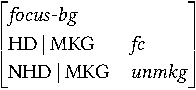
\includegraphics{pdf/focus-bg.pdf}}}}

\noindent This AVM serves to prevent constituents with information
structure markers from being used in cleft constructions. For
instance, \nun in \ili{Korean} is not allowed to be used in cleft
clauses, as exemplified in \myref{exe:kor:cleft:apple:7}.\is{clefting}


\myexe{\enumsentence{\label{exe:kor:cleft:apple:7}
\shortex{4}
  {Kim-i/*un & mek-nun & kes-un & sakwa-i-ta.}
  {Kim-\textsc{nom}/\textsc{nun} & eat-\textsc{rel} & thing-\textsc{nun} & apple-\textsc{cop}-\textsc{decl}}
  {`It is an apple that Kim is eating.' [kor]}}}

\noindent If a grammar employs a set of phrase structure rules that
transmit the MKG value of the subject in the cleft clause to the
higher phrase node, then only the nominative marker that involves [MKG
  \tdl{unmkg}] can be chosen.  The [MKG \tdl{tp}] feature \nun
involves prevents the clause from being used in the clefte clause (see
\myS{9:ssec:jpn:kor} \mypage{avm:ika:nun:kor}).


To present another instance, \tdl{narrow-focus} in Language \textit{A}
can be constrained as follows. Note that the values on HD and NHD are
the reverse of those in \myref{avm:focus-bg}.\is{narrow focus}

\myexe{\enumsentence{\label{avm:narrow-focus}\evnup{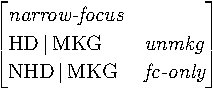
\includegraphics{pdf/narrow-focus.pdf}}}}

\noindent \myref{avm:narrow-focus} also explains the ungrammaticality
of pseudo sentence (\ref{exe:lang-a}c) in Language \textit{A}; HD of
\tdl{narrow-focus} requires a minus value as a value of MKG{$\mid$}FC,
which conflicts with a \isi{focus} accent that falls on the verb. Because
presumably there is no other way to construct (\ref{exe:lang-a}c), a
pseudo sentence like (\ref{exe:lang-a}c) remains ungrammatical.

\myexe{\eenumsentence{\label{exe:lang-a}
\item subj verb obj. (in the neutral word order)
\item subj obj verb. (focus on obj)
\item *subj obj \textsc{verb}. (a focus-marking accent on verb)}}


\noindent A sample derivation for (\ref{exe:lang-a}b) can be sketched
out as \myref{fig:lang-a}, showing only information
structure markings and sentential forms. Note that MKG is seen only
locally, because it is not a head feature. Thus, the value would not
be transmitted to the higher nodes if it were not for an extra
constraint.


\myexe{\enumsentence{\label{fig:lang-a}\evnup{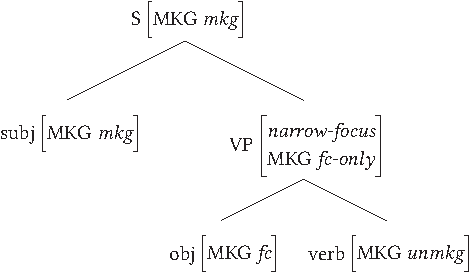
\includegraphics{pdf/lang-a.pdf}}}}


\tdl{Wide-focus},\is{wide focus} next, is particularly related to realization of
comment markers as mentioned earlier. For instance, Mandarin
\ili{Chinese} employs \textit{sh\`{i}} as exemplified below, which
indicates the remaining part after it is in the \isi{focus} domain
\citep{prince:12}.\footnote{\citet{prince:12} says this
  \textit{sh\`{i}} is different from the \isi{copula} \textit{sh\`{i}}
  (i.e.\ homonym).} In a similar vein, \citet{li:09} regards
\textit{sh\`{i}} as a marker responsible for contrastive meanings: The
constituents after \textit{sh\`{i}} are contrastively focused.\is{contrast}


\myexe{\enumsentence{\label{exe:shi:1}
\shortex{4} 
{Zh\={a}ngs\={a}n & [sh\`{i} & [xu\'{e}x\'{i} & y\={\i}xu\'{e}]].}
{Zhangsan & \textsc{shi} & study & medicine}
{`Zhangsan studies medicine.' [cmn] \citep[p.\ 336]{prince:12}}}}


\noindent Thus, the type of construction licensed by \textit{sh\`{i}}
(and comment markers in other languages such as \ili{Abma}
\citep{schneider:09}) has to inherit \myref{avm:wide-focus}.  Note
that this constraint is language-universal, unlike
\tdl{narrow-focus}.\is{narrow focus} In the context of \isi{grammar engineering} for
the \lingo \isi{Grammar Matrix} system, \myref{avm:wide-focus} is
encoded into \texttt{matrix.tdl}, while the AVM for \tdl{narrow-focus}
could be either empty or encoded in \texttt{mylang.tdl}.  In
accordance with \myref{avm:wide-focus}, any constituents after the
comment marker should not be topic-marked.

\myexe{\enumsentence{\label{avm:wide-focus}\evnup{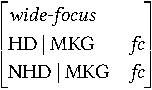
\includegraphics{pdf/wide-focus.pdf}}}}



\tdl{All-focus} inherits from both \tdl{wide-focus} and
\tdl{topicless}.\footnote{Regarding the status of \tdl{all-focus},
  \citet[p.\ 232]{lambrecht:96} argues that there is a clear
  difference from other types of focused constructions in that the
  pragmatic core of \tdl{all-focus} is ``an absence of the relevant
  presuppositions''.  The argument sounds convincing, but the present
  study does not represent such pragmatic information on the AVMs of
  \tdl{sform}.\is{sentential forms}\is{\textit{sform}}} Finally, it is
necessary to discriminate between \tdl{frame-setting} and
\tdl{non-frame-setting}.\is{topicless} As noted, this use of the MKG feature aims to
pass up appropriate values; in particular, when a topic-marked
constituent occurs in the leftmost
position. \mbox{[NHD{$\mid$}L-PERIPH +]} in (\ref{avm:frame-setting}a)
imposes this constraint.\is{frame-setting}\is{periphery}
\isi{L-PERIPH} (Left-PERIPHeral) will be discussed in the next chapter
(\myS{9:ssec:periphery}).



\myexe{\eenumsentence{\toplabel{avm:frame-setting}
\item\evnup{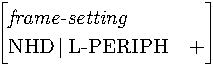
\includegraphics{pdf/frame-setting.pdf}}
\item\evnup{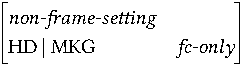
\includegraphics{pdf/non-frame-setting.pdf}}}}


\noindent As seen in Chapter~\ref{chapter3}
(\myS{3:sssec:multiple-topics}) topics that function to restrict the
frame of what the speaker is speaking about (i.e.\ so-called
\isi{frame-setting} topics) can appear multiply.\is{topic}

In \ili{English}, while left-dislocated NPs cannot occur more than
once without affecting grammaticality as shown in
(\ref{exe:multiple-topic:eng:2}a),\footnote{This generalization is
  language-specific, not universal.  Some counterexamples have been
  reported: \citet[p.\ 123]{vallduvi:93} argues on \ili{Catalan} that
  ``There is no structural restriction on the number of phrases that
  may be right or left detached.''  Left-dislocated NPs in
  \ili{Spanish} are also sometimes multiply used
  \citep[p.\ 224]{zagona:02}.}  frame-setters such as
\textit{yesterday} in (\ref{exe:multiple-topic:eng:2}b) can occur
multiple times in the sentence-initial position as presented in
(\ref{exe:multiple-topic:eng:2}d).\is{frame-setter} In other words,
\tdl{topic-comment} constructions can be used as another comment, and
do not constrain the value of MKG of the head-daughter.\is{topic-comment}
However, they cannot be used again for \tdl{non-frame-setting}.

 
\myexe{\eenumsentence{\label{exe:multiple-topic:eng:2}
\item{*Kim, the book, he read it.}
\item{Yesterday, Kim read the book.}
\item{The book, Kim read it.}
\item{Yesterday, the book, Kim read it.}}}



To sum up,\is{sentential forms} \tdl{sform} is concerned with
syntactic combination between two phrases with respect to information
structure.  This places constraints on both MKG and ICONS, relating
the marking to the meaning. In other words, \tdl{sform} makes
information structure marking and meaning interact with each other.
The type hierarchy here used is adapted from the proposal of
\citet{paggio:09}. The current proposal has one method in common with
\citeauthor{paggio:09}'s: If a phrase structure rule is related to
expressing information structure, it can multiply inherit from both a
specific type of \tdl{sform} and an ordinary phrase structure type,
such as \tdl{head-subj-phrase}, \tdl{head-comp-phrase}, etc. The main
difference between \citeauthor{paggio:09}'s approach and mine is that
my \tdl{sform} hierarchy does not directly constrain the linear order
of components.\is{\textit{sform}}



\section{Graphical Representation}
\label{9:sec:graph}


\citet{song:bender:12} suggest representing constraints on information
structure in the style of the dependency graphs of DMRS (Dependency
MRS; \citealt{copestake:09}) for ease of exposition.\is{MRS} Likewise,
the remainder of this book makes use of dependency graphs to present
information structure relations between individuals and clauses.

In these graphs, the \isi{ICONS} values are represented as links
between informatively contentful elements (introducing the referential
index as the value of TARGET) and verbs (introducing the event
variable as the value of CLAUSE) and as unary properties of verbs
themselves.\is{CLAUSE}\is{TARGET} The direction of a given arrow
stands for the \isi{binary relation} between a TARGET (an entity) and
a CLAUSE that the TARGET belongs to.  The start point indicates the
constituent that occupies the CLAUSE-KEY within the clause.  The end
point refers to the constituent whose INDEX is shared with the TARGET,
and whose ICONS-KEY{$\mid$}CLAUSE is co-indexed with the
CLAUSE-KEY.\is{ICONS-KEY} The node name on each arrow indicates the
information structure value that the binary relation has, such as
\tdl{focus}, \tdl{topic}, and so forth.\is{focus}\is{topic}

For example, a dependency graph (\ref{fig:sample:graph}b), which
stands for the binary relations on the ICONS list, is a shorthand
version of the corresponding MRS representation
(\ref{fig:sample:graph}a), which stands for \textit{\textbf{Kim} reads
  the \textsc{book}}. in which the B-accented \textit{\textbf{Kim}}
conveys meaning of contrast and/or topic,\is{B-accent} and the
A-accented \textit{\textsc{book}} bears non-contrastive
\isi{focus}.\is{A-accent}\is{B-accent}\is{contrast}


\myexe{\eenumsentence{\label{fig:sample:graph}
\item\evnup{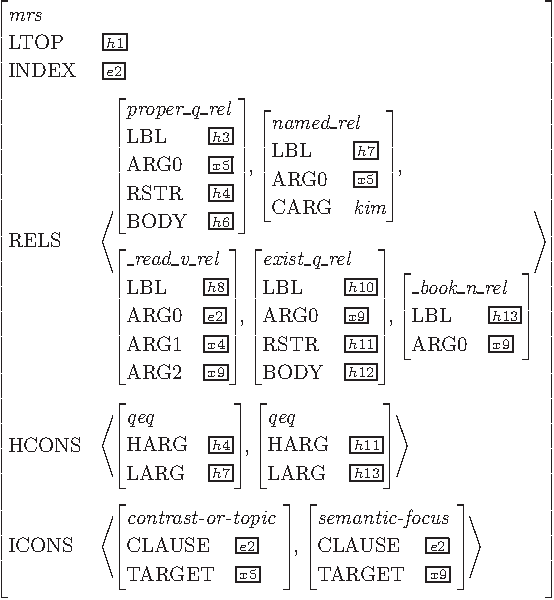
\includegraphics{pdf/sample-mrs.pdf}}
\item\evnup{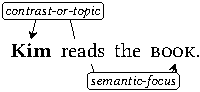
\includegraphics{pdf/sample-graph.pdf}}}}


\noindent The arc from \textit{reads} to \textbf{Kim} means that the
index of \textbf{Kim} has a \tdl{contrast-or-topic} relation to the
clause represented by \textsc{reads}.\footnote{The present
  study, according to the argument of \citet{hedberg:06}, regards the
  A-accent (i.e.\ marked as \textsc{small caps}) as prosodic means
  expressing \isi{non-contrastive focus} (i.e.\ \tdl{semantic-focus}),\is{semantic focus}
  and  the B-accent (i.e.\ \textbf{boldfaced}) as conveying one of the
  meanings of \isi{non-contrastive topic}, \isi{contrastive topic}, or sometimes
  \isi{contrastive focus}.} The arc from \textit{reads} to \textsc{book},
likewise, means the index of \textsc{book} has a \tdl{semantic-focus}
relation to the index of \textsc{reads}.\is{semantic focus} The root arrow on
\textsc{reads} indicates that the verb is linguistically
underspecified with respect to the clause that it heads.



\section{Summary}
\label{9:sec:summary}

This chapter has outlined three considerations motivating the
representation of information structure via ICONS: resolving
discrepancies between forms and meanings in information structure,
facilitating underspecifiability for allowing flexible and partial
constraints,\is{underspecification} and capturing the fact that
information structure relations are between expressions and particular
clauses.  Additionally, the ICONS-based representation reflects the
working hypothesis that semantically empty and syncategorematic items
are informatively empty.  Guided by these considerations, I provide
three type hierarchies: \tdl{info-str} whose value types stratify
information structure meaning, \tdl{mkg} indicating morphosyntactic
markings of information structure,\is{MKG}\is{\textit{mkg}} and
\tdl{sform} that works with MKG relating to the \tdl{info-str}
value.\is{sentential forms}\is{\textit{sform}} \isi{ICONS} is added
into \tdl{mrs}, and the value is a \tdl{diff-list} of \tdl{info-str}.
\isi{ICONS} identifies which element has which information structure
relation to which clause. For this purpose, the typed feature
structure of \tdl{info-str} includes TARGET and
CLAUSE.\is{CLAUSE}\is{TARGET} TARGET is identified with the EP's INDEX
(i.e.\ \tdl{individual}), and CLAUSE is determined by the subtype(s)
of \tdl{clause}.\is{ICONS-KEY} In addition, ICONS-KEY and CLAUSE-KEY
are used as pointers during the construction of parse trees.  MKG has
two features; one is FC (FoCus-marked), and the other is TP
(ToPic-marked). These features are independent of meanings represented
as an \tdl{info-str} type.  The next chapter will discuss how these
elements are used to impose constraints on information structure and
represent it in MRS.\is{MRS}























